\documentclass[10pt,a4paper]{article}
\usepackage[utf8]{inputenc}
\usepackage{amsmath}
\usepackage{amsfonts}
\usepackage{amssymb}
\usepackage{geometry}
\usepackage{verbatim}
\usepackage{enumerate}
\usepackage{fancyvrb}
\usepackage{graphicx}
\usepackage{tikz}
\usepackage{hyperref}
\usetikzlibrary{positioning}
\usetikzlibrary{shapes,snakes}
\usepackage[english]{babel}

\geometry{legalpaper, margin=1.5in}

\author{William Schultz}
\begin{document}
\title{Program Synthesis}
\author{William Schultz}
\maketitle

% \section{Reactive synthesis}

In general, we can present the \textit{synthesis} problem in contrast to the verification problem as follows:
\begin{itemize}
    \item The \textbf{verification problem}: given system $M$ and spec $\varphi$, check that $M \vDash \varphi$.
    \item The \textbf{synthesis problem}: given spec $\varphi$, find $M$ such that $M \vDash \varphi$.
\end{itemize}

\subsection{Functional Synthesis}

The classic, \textit{functional synthesis} problem, is defined with respect to programs that take some input $x$ and transform it to output $y$. In this setting, if we are given a specification $\varphi$ that prescribes the desired input/output relation, we can construct a program by means of establishing validity of the theorem
\begin{align*}
    \forall x \, \exists y : \varphi(x,y)
\end{align*}
Note that this is equivalent to the second order formula
\begin{align*}
    \exists f, \forall x : \varphi(x,f(x))
\end{align*}
where $f$ is a concrete function that takes input $x$ and returns the correct output $y$ satisfying specification $\varphi$ \cite{1989pnuelirosner,1969waldingersynthprow}. If we have a constructive way to prove this theorem, then we can construct $f$, from which we can construct a program that satisfies $\varphi$. This approach is also referred to as \textit{deductive synthesis} \cite{manna1980deductive}.

\subsection{Reactive Synthesis}

The above approach is suitable for sequential programs, but if we want to move to concurrent programs, then we need a more expressive specification language in which to express $\varphi$. Temporal logic became the natural choice for this and the works of \cite{1981clarkemerson, 1984mannawolper} essentially do concurrent program synthesis by showing satisfiability of of a particular temporal formula specification $\varphi$, and then using the model satisfying $\varphi$ to construct a program implementing $\varphi$.

In \cite{1989pnuelirosner}, however, they claim that the approach taken in \cite{1981clarkemerson, 1984mannawolper} is not quite sufficient, because it assumes that we are trying to synthesize \textit{closed} systems. That is, systems for which we have full control over every component. They claim that if, for example, we aree synthesizing a system with two components, $C_1$ and $C_2$, the ``hidden assumption'' in \cite{1981clarkemerson} is that we have the power to construct both $C_1$ and $C_2$ in a way that will ensure the needed cooperation. But, if we are in a so-called \textit{open system} setting, then $C_1$, for example, may represent the \textit{environment} over which the implementor has no control, while $C_2$ is the body of the system itself (which we may refer to as a \textit{reactive module}). In this case, we instead have to synthesize $C_2$ in such a way that it will work correctly in response to any possible behaviors of the environment $C_1$. 

For example, if $C_1$ is a module that can only modify $x$ (a shared variable for communication), and $C_2$ can only modify $y$, then they claim the synthesis problem should instead be stated as
\begin{align*}
    \forall x \, \exists y : \varphi(x,y)
\end{align*}
which they refer to as the \textit{reactive synthesis} problem. Note that in the formal statement above, we should now interpret $x$ and $y$ as being quantified over behaviors of the computation, since we are now interpreting it over temporal logic. So, the statement is saying that for any possible sequence of values $x$ (that can be produced by the environment $C_1$), there exists a sequence of values $y$ (produced by the controllable system $C_2$) such that $\varphi(x,y)$ holds. They note that the approach of \cite{1981clarkemerson} can be viewed as a solution to the alternate problem statement $\exists x \, \exists y : \varphi(x,y)$.

\subsection{Temporal Synthesis}

\textit{Temporal synthesis} considers specifications given in the form of LTL (or CTL), for example. An initial approach was to use satisfiability of a temporal formula as a way to derive $M$ \cite{1981clarkemerson}. 
See also \cite{1984mannawolper}. 

In \cite{1981clarkemerson} they consider concurrent systems consisting of a finite number of fixed processes $P_1,\dots,P_m$ running in parallel. They treat parallelism in the usual sense i.e. non-deterministic interleaving of the sequential atomic actions of each process. They use CTL as a specification language, and consider the semantics of CTL with respect to a (Kripke) structure $M=(S,A_1,\dots,A_k,L)$, where
\begin{itemize}
    \item $S$: countable set of system states
    \item $A_i \subseteq S \times S$: transition relation of process $i$
    \item $L$: assignment of atomic propositions to each state
\end{itemize}
They use a decision procedure for satisfiability of CTL formulae (similar to one described in \cite{1981benari}) as part of their synthesis procedure. Given a CTL formula $f_0$, the decision procedure returns either ``Yes, $f_0$ is satisfiable or ``No, $f_0$ is unsatisfiable''. If $f_0$ is satisfiable, then a finite model (structure) is also constructed. Their overall synthesis algorithm consists of the following high level steps:
\begin{enumerate}
    \item Specify the desired behavior of the concurrent system using a CTL formula $\varphi$.
    \item Apply the decision procedure to the formula $\varphi$ to obtain a finite model of the formula.
    \item Factor out the synchronization skeletons of the individual processes from the global system flowgraph defined by the model.
\end{enumerate}
They demonstrate this procedure on a simple, 2 process mutual exclusion example. Below is shown the description of the abstract states of each process, $\{NCS_i, TRY_i, CS_i\}$: 
\begin{center}
    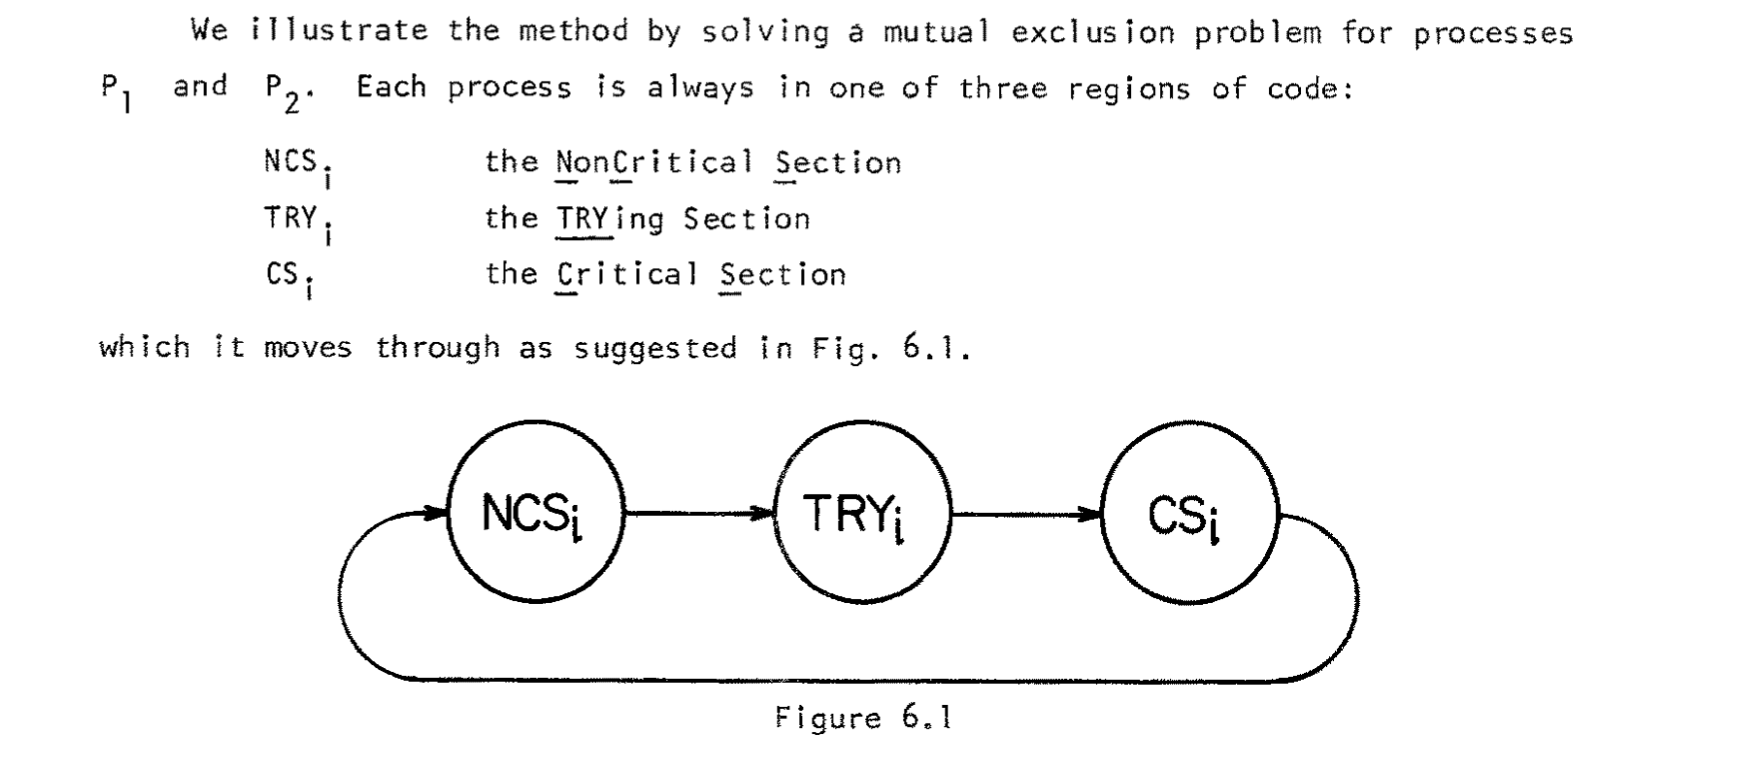
\includegraphics[scale=0.4]{images/mutex_processes.png}
\end{center}
and they give the specification of the mutual exclusion problem in CTL as follows:
\begin{center}
    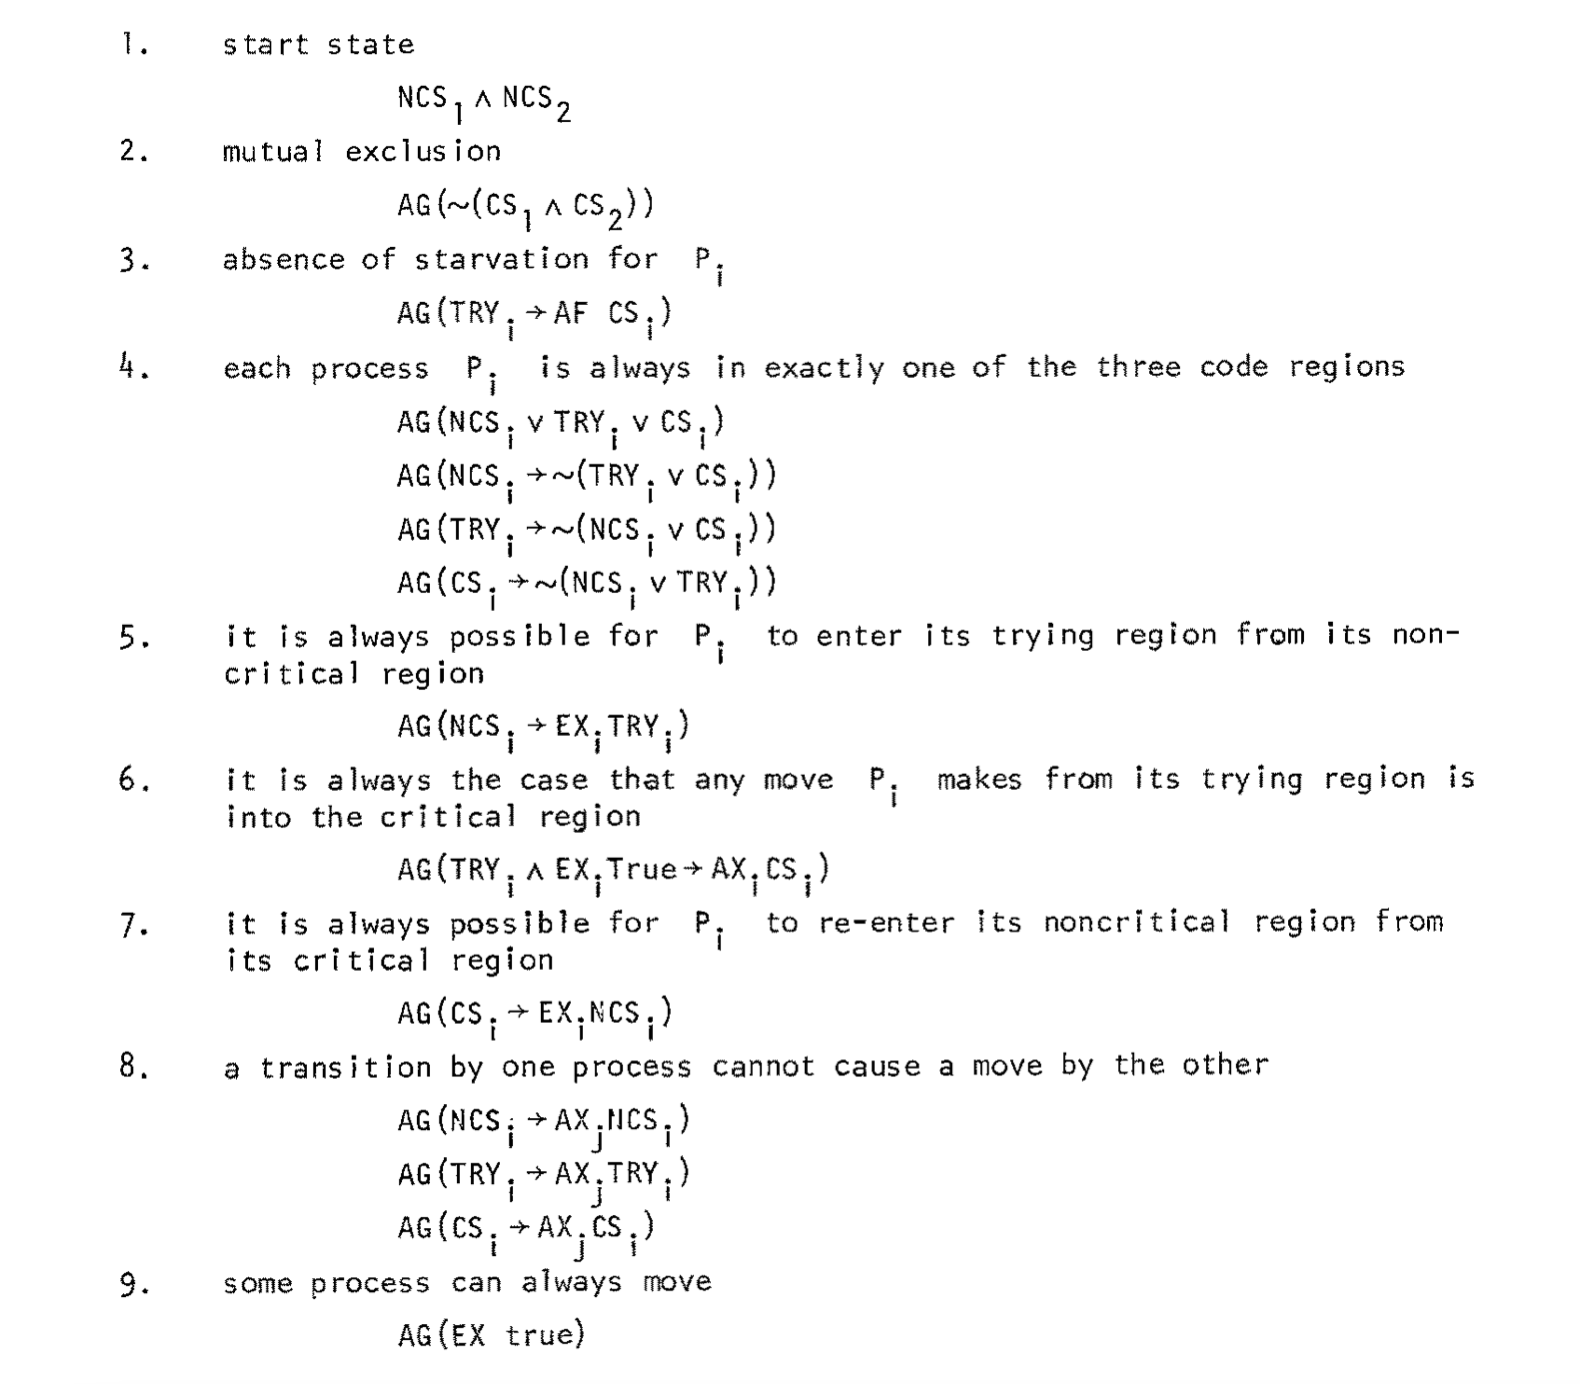
\includegraphics[scale=0.45]{images/mutex_spec.png}
\end{center}
From this they then construct a tableau $T$ using their decision procedure:
\begin{center}
    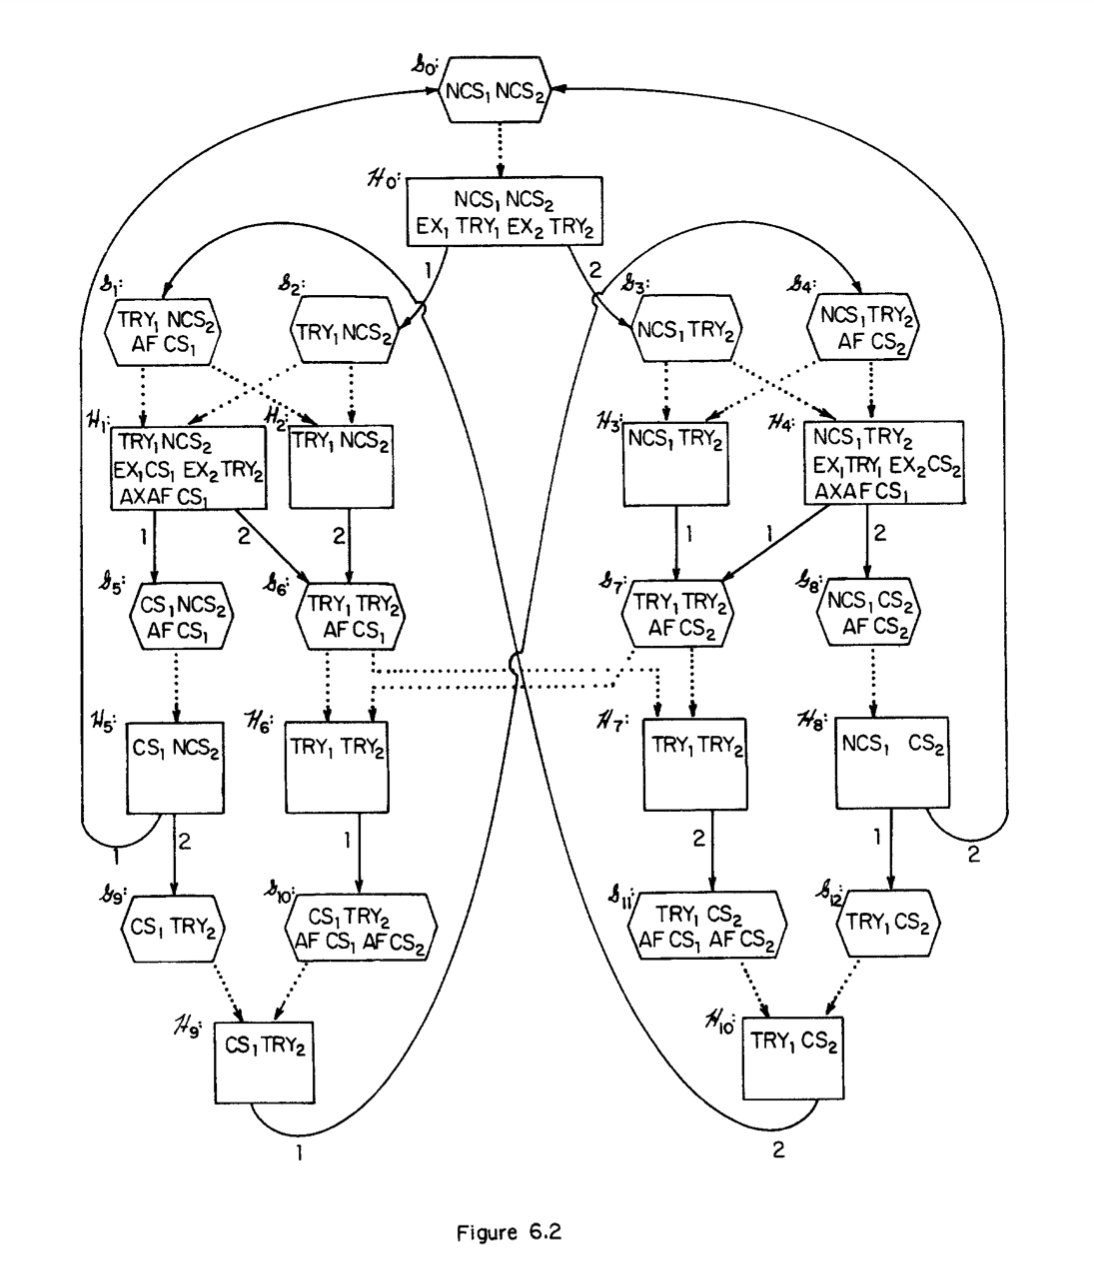
\includegraphics[scale=0.4]{images/mutex_tableau.png}
\end{center}
and then from $T$ they extract a finite model of the global program behavior:
\begin{center}
    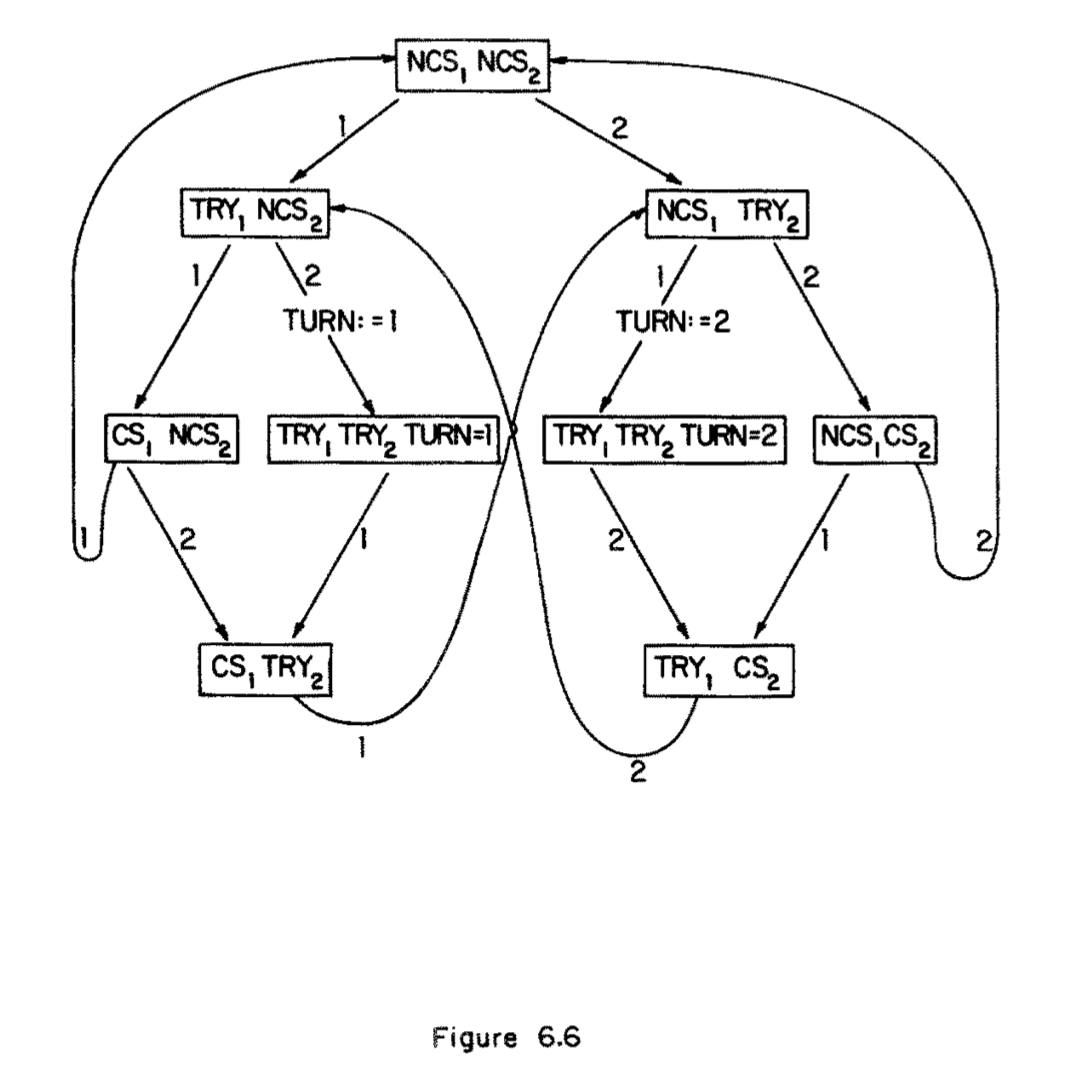
\includegraphics[scale=0.4]{images/mutex_model.png}
\end{center}
Note they manually introduced an auxiliary variable $TURN$ in order to distinguish states $H_6$ and $H_7$ in the tableau, which carries over into the extracted model. 

After constructing the model representing the global program behavior, they extract ``skeletons'' for each individual process, which they seem to describe in a somewhat ad hoc manner i.e. they don't give a formal algorithmic procedure for this. Note that this is pointed out in \cite{2001attie}, which appears to give a more formal treatment of this extraction procedure. The final, extracted skeletons for process $P_1$ and $P_2$ are shown as follows:
\begin{center}
    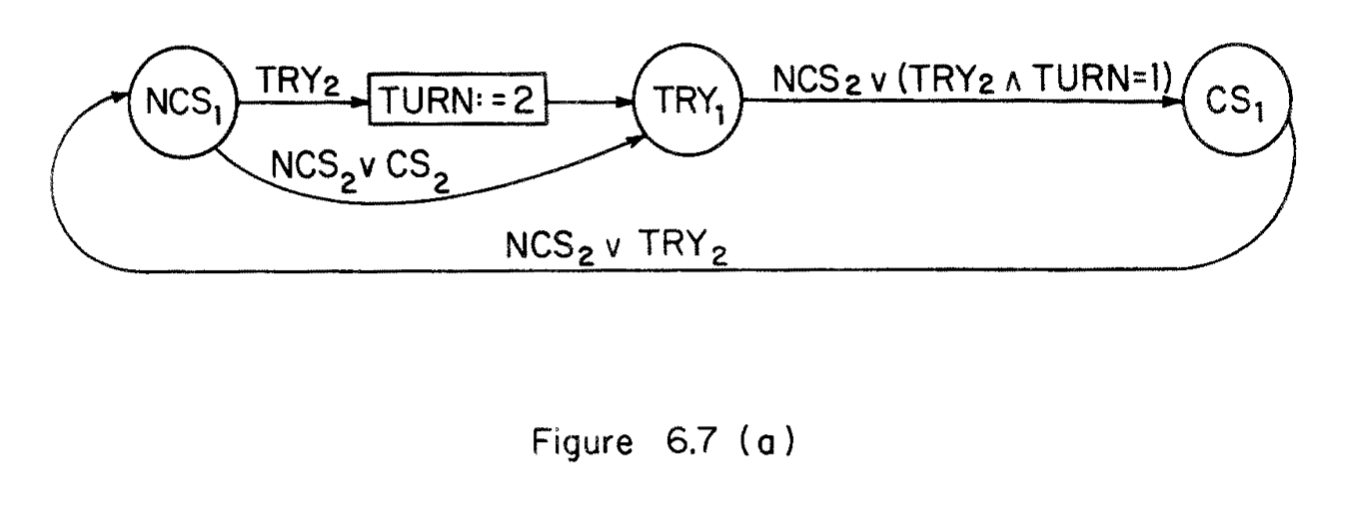
\includegraphics[scale=0.3]{images/mutex_p1.png}
\end{center}
\begin{center}
    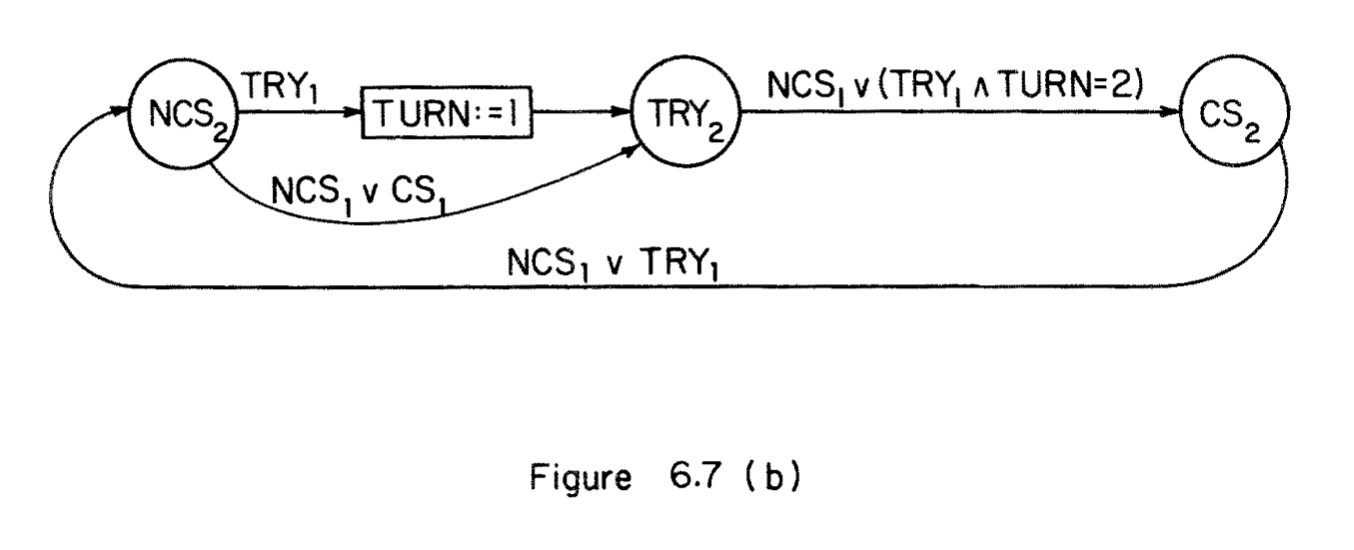
\includegraphics[scale=0.3]{images/mutex_p2.png}
\end{center}

% \bibliographystyle{plain}
\bibliographystyle{alpha} 
\bibliography{../../references.bib}

\end{document}